%%
%% This is file `sample-sigconf.tex',
%% generated with the docstrip utility.
%%
%% The original source files were:
%%
%% samples.dtx  (with options: `sigconf')
%% 
%% IMPORTANT NOTICE:
%% 
%% For the copyright see the source file.
%% 
%% Any modified versions of this file must be renamed
%% with new filenames distinct from sample-sigconf.tex.
%% 
%% For distribution of the original source see the terms
%% for copying and modification in the file samples.dtx.
%% 
%% This generated file may be distributed as long as the
%% original source files, as listed above, are part of the
%% same distribution. (The sources need not necessarily be
%% in the same archive or directory.)
%%
%% The first command in your LaTeX source must be the \documentclass command.
\documentclass[sigconf]{acmart}

%%
%% \BibTeX command to typeset BibTeX logo in the docs
\AtBeginDocument{%
	\providecommand\BibTeX{{%
			\normalfont B\kern-0.5em{\scshape i\kern-0.25em b}\kern-0.8em\TeX}}}

%% Rights management information.  This information is sent to you
%% when you complete the rights form.  These commands have SAMPLE
%% values in them; it is your responsibility as an author to replace
%% the commands and values with those provided to you when you
%% complete the rights form.

%% --------------------------- NOT NEEDED --------------------
\setcopyright{none}
\copyrightyear{2019}
\acmYear{2019}
\acmDOI{none}

%% These commands are for a PROCEEDINGS abstract or paper.
\acmConference[Ambient Computing Seminar]{Lübeck '19: Using Wearables to Support Sports Training}{June 07, 2019}{}
%\acmBooktitle{Woodstock '18: ACM Symposium on Neural Gaze Detection,
%  June 03--05, 2018, Woodstock, NY}
%\acmPrice{15.00}
%\acmISBN{978-1-4503-9999-9/18/06}


\usepackage[T1]{fontenc}
\usepackage{lmodern}

%%
%% Submission ID.
%% Use this when submitting an article to a sponsored event. You'll
%% receive a unique submission ID from the organizers
%% of the event, and this ID should be used as the parameter to this command.
%%\acmSubmissionID{123-A56-BU3}

%%
%% The majority of ACM publications use numbered citations and
%% references.  The command \citestyle{authoryear} switches to the
%% "author year" style.
%%
%% If you are preparing content for an event
%% sponsored by ACM SIGGRAPH, you must use the "author year" style of
%% citations and references.
%% Uncommenting
%% the next command will enable that style.
%%\citestyle{acmauthoryear}

%%
%% end of the preamble, start of the body of the document source.
\begin{document}
	
	%%
	%% The "title" command has an optional parameter,
	%% allowing the author to define a "short title" to be used in page headers.
	\title{Using Wearables to Support Sports Training}
	
	%%
	%% The "author" command and its associated commands are used to define
	%% the authors and their affiliations.
	%% Of note is the shared affiliation of the first two authors, and the
	%% "authornote" and "authornotemark" commands
	%% used to denote shared contribution to the research.
	\author{Alexander Andreevi\v{c} Osiik}
	\affiliation{%
		\institution{University of L\"ubeck}
		\country{Germany}
	}
	\email{alexander.osiik@student.uni-luebeck.de}
	
	%%
	%% By default, the full list of authors will be used in the page
	%% headers. Often, this list is too long, and will overlap
	%% other information printed in the page headers. This command allows
	%% the author to define a more concise list
	%% of authors' names for this purpose.
	\renewcommand{\shortauthors}{A.A. Osiik}
	
	%%
	%% The abstract is a short summary of the work to be presented in the
	%% article.
	\begin{abstract}
		Over the past few years, wearable technologies have gained increasing popularity and acceptance \cite{Trend}. With the progress of technology, sensor nodes are becoming smaller, lighter and more reliable, meaning that the corresponding wearable devices can be worn imperceptebly by athletes. These divices shall not interfere with an athlete's sports locomotion. On the other hand, depending on application area, these devices must be noticeable enough to give unambiguous feedback at specific time points, enhancing the sports experience.
		In this paper, a report on the state of the art of wearabe technologies in sports is provided. Various approaches for different types of sports or sports movements are introduced, evaluated and compared under the aspect of usability.
	\end{abstract}
	
%	%%
%	%% The code below is generated by the tool at http://dl.acm.org/ccs.cfm.
%	%% Please copy and paste the code instead of the example below.
%	%%
%	\begin{CCSXML}
%		<ccs2012>
%		<concept>
%		<concept_id>10010520.10010553.10010562</concept_id>
%		<concept_desc>Computer systems organization~Embedded systems</concept_desc>
%		<concept_significance>500</concept_significance>
%		</concept>
%		<concept>
%		<concept_id>10010520.10010575.10010755</concept_id>
%		<concept_desc>Computer systems organization~Redundancy</concept_desc>
%		<concept_significance>300</concept_significance>
%		</concept>
%		<concept>
%		<concept_id>10010520.10010553.10010554</concept_id>
%		<concept_desc>Computer systems organization~Robotics</concept_desc>
%		<concept_significance>100</concept_significance>
%		</concept>
%		<concept>
%		<concept_id>10003033.10003083.10003095</concept_id>
%		<concept_desc>Networks~Network reliability</concept_desc>
%		<concept_significance>100</concept_significance>
%		</concept>
%		</ccs2012>
%	\end{CCSXML}
%	
%	\ccsdesc[500]{Computer systems organization~Embedded systems}
%	\ccsdesc[300]{Computer systems organization~Redundancy}
%	\ccsdesc{Computer systems organization~Robotics}
%	\ccsdesc[100]{Networks~Network reliability}
	
	%%
	%% Keywords. The author(s) should pick words that accurately describe
	%% the work being presented. Separate the keywords with commas.
	\keywords{wearables, pervasive computing, ubiquitous computing, sports}
	
	%% A "teaser" image appears between the author and affiliation
	%% information and the body of the document, and typically spans the
	%% page.
	\begin{teaserfigure}\centering
		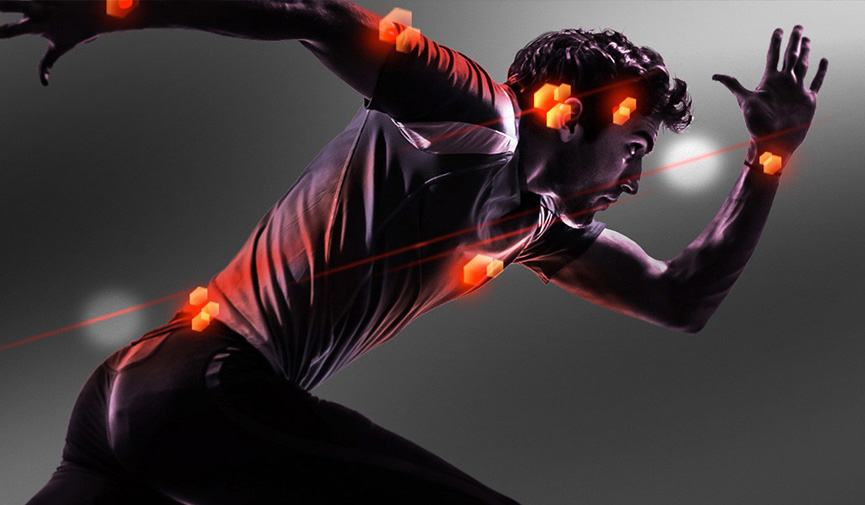
\includegraphics[width=12cm]{Images/wearables.jpg}
		\caption{Improved smart wearables for sensing in sports \cite{Cruyff}}
		\label{fig:teaser}
	\end{teaserfigure}
	
	%%
	%% This command processes the author and affiliation and title
	%% information and builds the first part of the formatted document.
	\maketitle
	
	\section{Introduction}
		\par The electronic wearable market’s challenge is to create devices that can offer useful data that will improve our lives. Whether worn on the wrist, head or foot, wearables must be fashionable, rugged, and easily rechargeable \cite{TE}.   
		\par 
		This means that sports technology is trying to become less noticeable,  while getting increasingly important in recent years. It is important, that the improvement of sports technology not only means improvement of training surface (better track, fields), equipment (lighter, while more robust equipment), and clothing (specified for various weather conditions), but also improvement and wider use of computer assisted technology.
		Some technologies must be as imperceptable as possible, otherwise, through Observer Effect, one athletes awareness oft he system will impact ist performance.
		\par 
		Sports technologies will concentrate on wearables (the computer is on the user) or objects used for sports (the computer is on a needed piece of equipment)
		Instances for wearables: FitBit fitness bracelet or Hexoskin mart clothing, measuring Heart Rate, Breathing Rate, Breathing Volume. Might also be used in dangerous environment outside of the context of sports, f.i. firefighters and soldiers. GolfTEC and K-VEST for golfing.
		Instances for objects: Adidas miCoach smart soccer ball, tracking speed, spinrate, strikes and flightpath oft he ball, and bringing it to an App.
		
		State oft the Art:
		For werable devices in sports training, the most focus lies on data collection. Data from a specific extremety is collected, processed, and evaluated. The processed data will be used to teach „einen Leitfaden geben“ to a specific sports technique or motion pattern, optimize the userss performance and fitness level.
		\begin{itemize}
			\item What limbs to Track? 
			\item Where to put the Sensor?
			\item What group?
		\end{itemize}
			
			
			
		Faciliating instead of dictating. Wearable technologies should replace or be at least as good as a personal coach, consulting the user/athlete about better movement.
		Hardware is a hard choice. If it is too bulky, the device might not be accepted by athletes, as it is interfering. If it is highly flexible and ha slow profile, cable breaks might happen more often.
		Energy Harvesting plays a huge part in the success of wearable technologies. It is more than clear, that long term adoption of certain technologies might be reduced, if the technology hast o be charged too often, or the charging processed is combined with stress.
		
		Wearable technologies can be used for person groups, who can not afford a personal trainer, or are unable to move to a specific sports training environment due to body conditions. This might be very useful for elderly people or invalides, for whom leaving the house is combined with social and physical strain.


	\section{Use cases} 
		As shown in \cite{PervasiveComputing}, the current research of pervasive computing in sports technologies can be divided into three areas, namely athletic performance, entertainment, and how innovation changes the rules of the game. In this section, the focus will be solely on the first mentioned point, as the other two points will be fundamental topics of Section \ref{sec:Discussion}.
		
		\subsection{Wearables as personal coaching replacement}
		Good expertise, coaching, and adequate training equipment are not financially sustainable for everyone \cite{PersonalTrainer}.
		Therefore, one goal is to create a low cost training facility which is as professional as possible and does not necesserily need the longterm supervision of an expert coach. Use of wearable devices replaces stationary and bulky laboratory machines used by researchers \cite{SportSensing}. As the device is replacing a personal trainer, it must be perceived by the trainee in some way.
		
		\par A unique all-in-one 3D recording, analysis and sports training device is the K-VEST \cite{KVEST}. The K-Motion uses three wireless sensors located on the golfer’s hip, shoulder, and hand, aswell as video recording cameras for visual analysis. The training software then measures and analyzes the efficiency and movement pattern of the user's swing in real time, and gives visual feedback by showing the motion on a display. It is promised that the system is enhancing the user's training by showing the objective video footage, which is rendered within seconds, while high-speed cameras would take days or weeks to analyze a golf swing. It can detect errors in real time and the trainees can immediately implement the necessary changes to the swing \cite{KVEST2}.
		
		\par A similar approach is used in archery \cite{EArchery}. In this prototype, the user wears a glove with built in accelerometers tracking hand motion in order to capture the archer's release. This low-cost device classifies the archer's release into three possible outputs with a unique feedback signal, respectively. However, this approach differs somewhat from the example given above, namely in terms of preliminary work. As every archer has a unique body type and different muscular deveopment, this product's classifier, and the future user, must undergo a training process creating 50 release samples, supervised and labeled by a coach. This makes every E-Archery Glove unique for every user, which is the opposite of the above mentioned ``Plug-and-Play'' product.
		
		\subsection{Wearables as monitoring enhancement}
		In the section above, technology examples have been selected based on the premise that the user of the wearable device is the one interacting directly with it or receiving feedback from it. However, most professional athletes have a designated trainer, who either analyzes motion patterns and corrects them in the right way, or makes tactical decisions in game situations. In this case, the devices must be as imperceptable as possible for the players \cite{SportSensing}, and on the other hand the information collected must be as precise as possible for the trainer.
		
		\par The most popular and widespread types of sport in the world are usually team sports \cite{Popularity}. In sports like football, all team members act together towards a shared objective, while being led by a single coach or a coaching staff, taking responsibility for tactical decisions. A wearable device-based framework is introduced in \cite{FootballPitch}, which provides each player with a sensor capable of storing GPS data, amount of steps and heart rate. The sensors are connected to a cloud server, where a classifier evaluates the data and passes on the current physical state of a player to the trainer. This product consults the trainer, depending on the current game situation, whether to substitute a fatigued player or not. This is a crucial decision, as fatigue is considered as the second highest injury risk in sports. While the amount of substitutions per game is usually limited in football, this prototype framework can be even more effective in sports like handball or american football, where substitutions can occur limitless at any point of the game.
		
		\begin{figure}[t]\centering
			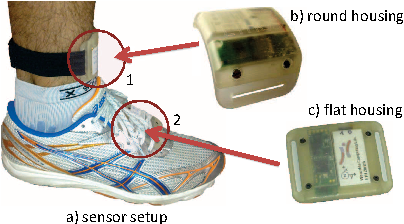
\includegraphics[width=6cm]{Images/Figure1.png}
			\caption{Runner equipped with ETHOS devices \cite{InToTheWoods}}
			\label{fig:woods}
		\end{figure}
	
		\par For individual sports, a wearable device was tested in a user study in \cite{InToTheWoods}. Participants were equipped with ETHOS sensor nodes in various placements on the legs, see Figure \ref{fig:woods}. Thereafter, the tireness of muscle areas on an exhausting run is analyzed, based on the running movement. The data acquired in a run period is analyzed and evaluated afterwards, and can be used for research purposes or, in case of injury, doctor appointments.
		  
	
	\section{Limitations and Difficulties}
	Innovative wearable technologies must establish themselves regarding not only social aspects, such as broad acceptance by users, but also regarding physical endurance of hardware. To avoid the ``Observer Effect'' described above, the hardware profile of the wearable device must be kept as flat as possible, while still being robust enough to withstand high forces without tearing apart. 
	\par In \cite{SportSensing}, challenges of perfect hardware design are illustrated. Various sensors materials and communication methods were tested for an computer-equipped sprinting shoe, with successful and failed results. 
	
	 In \cite{PervasiveComputing}, social acceptance of technologies is discussed under consideration of rule changes of sports or experience enhancement for spectators. At present time, no computing enhancements are allowed to be used in many kinds of sport, since this offends against the rules. Allowing ``performance enhancing computing'' in sports may sooner or later chenge the rules of a specific sport, in extreme cases creating a completely new one, while erasing the other. This will be further discussed in section \ref{sec:Discussion}
	 
	 \begin{figure}\centering
	 	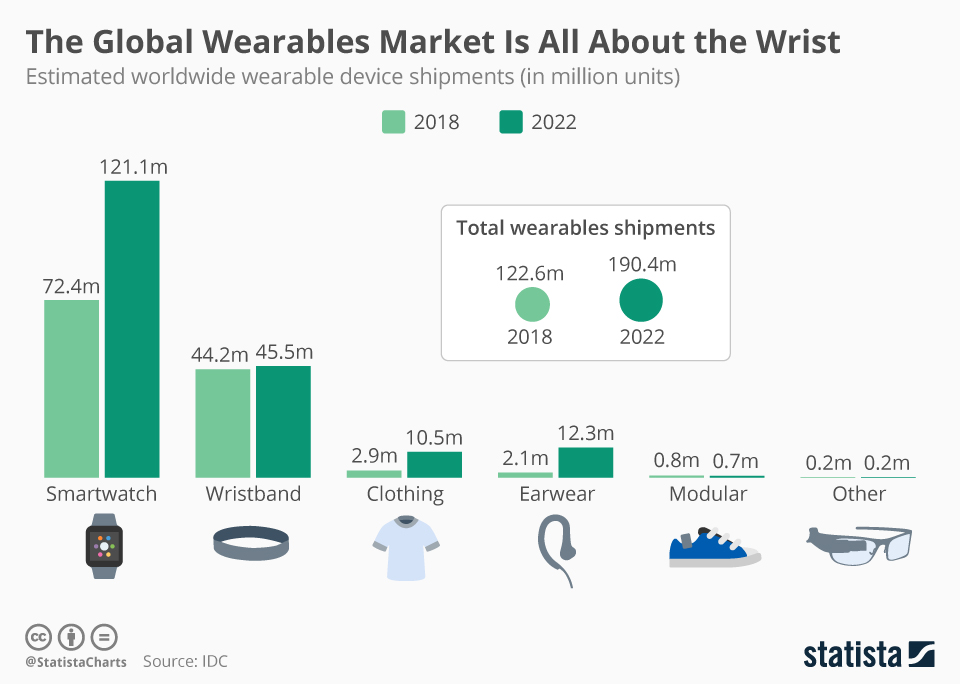
\includegraphics[width=8cm]{Images/Statista.jpg}
	 	\caption{This chart shows a forecast of worldwide wearable device shipments.  \cite{Statista}}
	 	\label{fig:Statista}
	 \end{figure}
 
	\section{Discussion}\label{sec:Discussion}
	In the previous sections we have discussed different approaches to wearable technologies for different sports. 
	- Regarding trend of wearable technologies...
	- Change Rules of Sports
	- Money Making for those, who can afford it
	- Practice may be cheaper (what if classifiers don't work Correctly?)
	
	
	
	
	VAR, Statistiken sind interessant, möglichst ohne Änderung des Spiels
	
	%%
	%% The acknowledgments section is defined using the "acks" environment
	%% (and NOT an unnumbered section). This ensures the proper
	%% identification of the section in the article metadata, and the
	%% consistent spelling of the heading.
%	\begin{acks}
%		To Robert, for the bagels and explaining CMYK and color spaces.
%	\end{acks}
	
	%%
	%% The next two lines define the bibliography style to be used, and
	%% the bibliography file.
	\bibliographystyle{ACM-Reference-Format}
	\bibliography{SeminarReferences}

	
\end{document}
\endinput
%%
%% End of file `sample-sigconf.tex'.
